\subsection{Componenti di Navigazione (Frontend)}

\subsubsection{Descrizione}
Il modulo di navigazione realizza l'albero gerarchico del DIP ed e il punto di ingresso principale per la consultazione delle entita archivistiche. La gerarchia visualizzata segue il modello:
\begin{center}
DIP -> DocumentClass -> Process -> Document -> File
\end{center}

L'implementazione segue una separazione netta delle responsabilita:
\begin{itemize}
	\item \textbf{Facade Pattern}: \textit{DipFacade} coordina stato, caricamenti e retry.
	\item \textbf{Gateway Pattern}: \textit{IpcGateway} incapsula la comunicazione IPC con il backend.
	\item \textbf{Smart/Dumb Components}: componenti smart per orchestrazione, componenti dumb per sola presentazione del nodo.
	\item \textbf{State reattivo}: la UI reagisce ai cambiamenti di stato di root, cache, loading e errori locali.
\end{itemize}

\subsubsection{Diagrammi condivisi (C1/C2/C3)}

\begin{figure}[H]
	\centering
	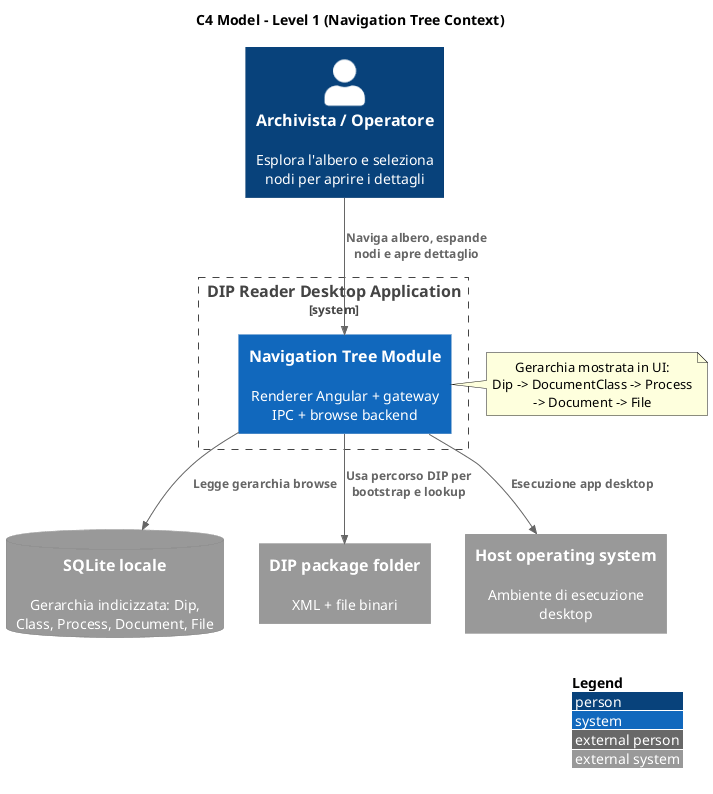
\includegraphics[width=0.85\textwidth]{../../assets/outDiagrammiST/C4_Navigation_Context.png}
	\caption{Diagramma C1 - System Context del modulo Albero di Navigazione}
	\label{fig:navigation:c1-context}
\end{figure}

\begin{figure}[H]
	\centering
	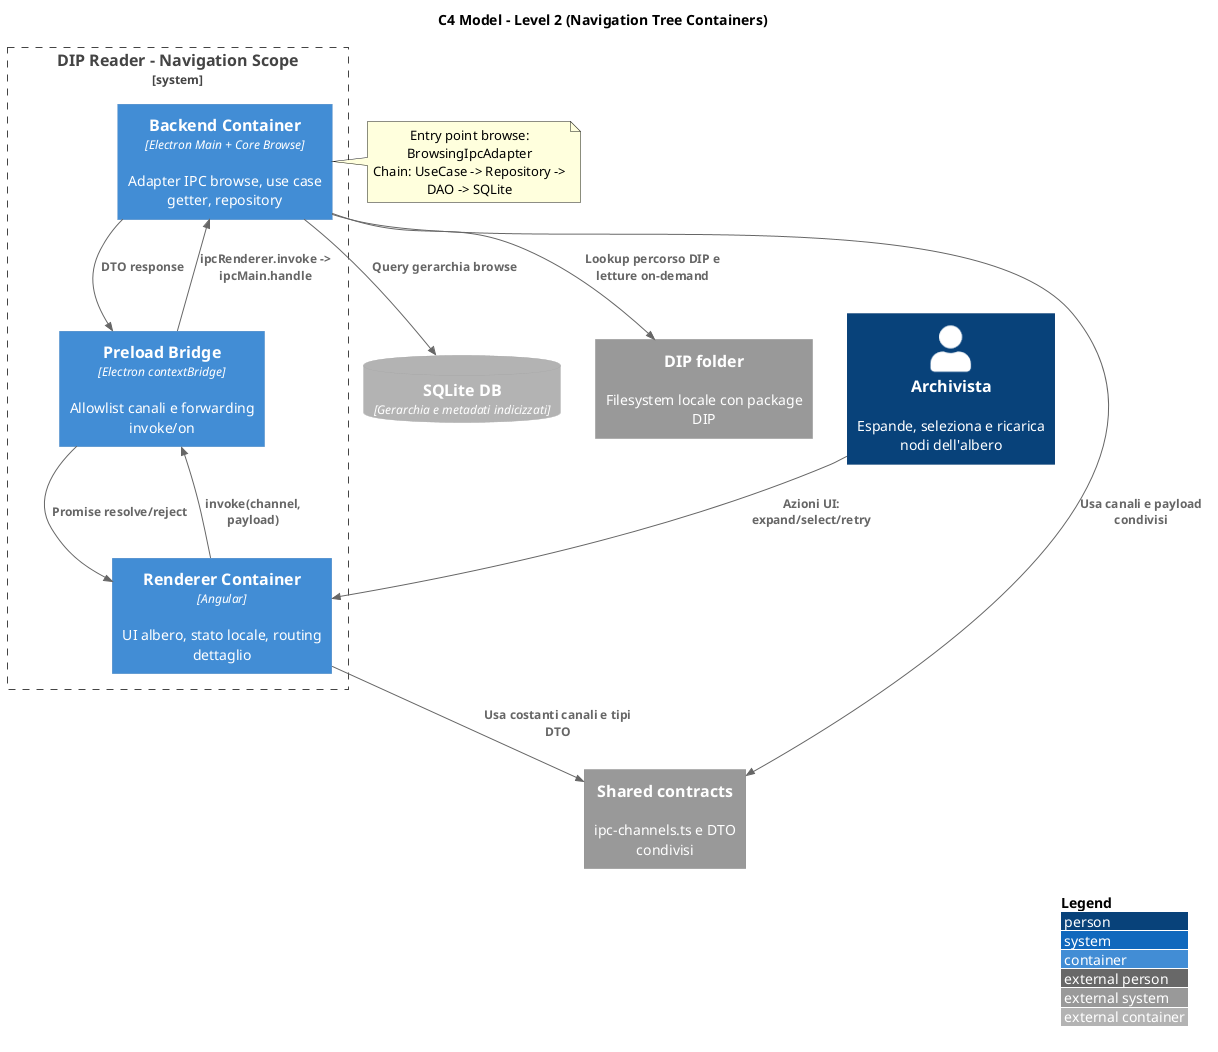
\includegraphics[width=0.85\textwidth]{../../assets/outDiagrammiST/C4_Navigation_Container.png}
	\caption{Diagramma C2 - Container View del modulo Albero di Navigazione}
	\label{fig:navigation:c2-container}
\end{figure}

\begin{figure}[H]
	\centering
	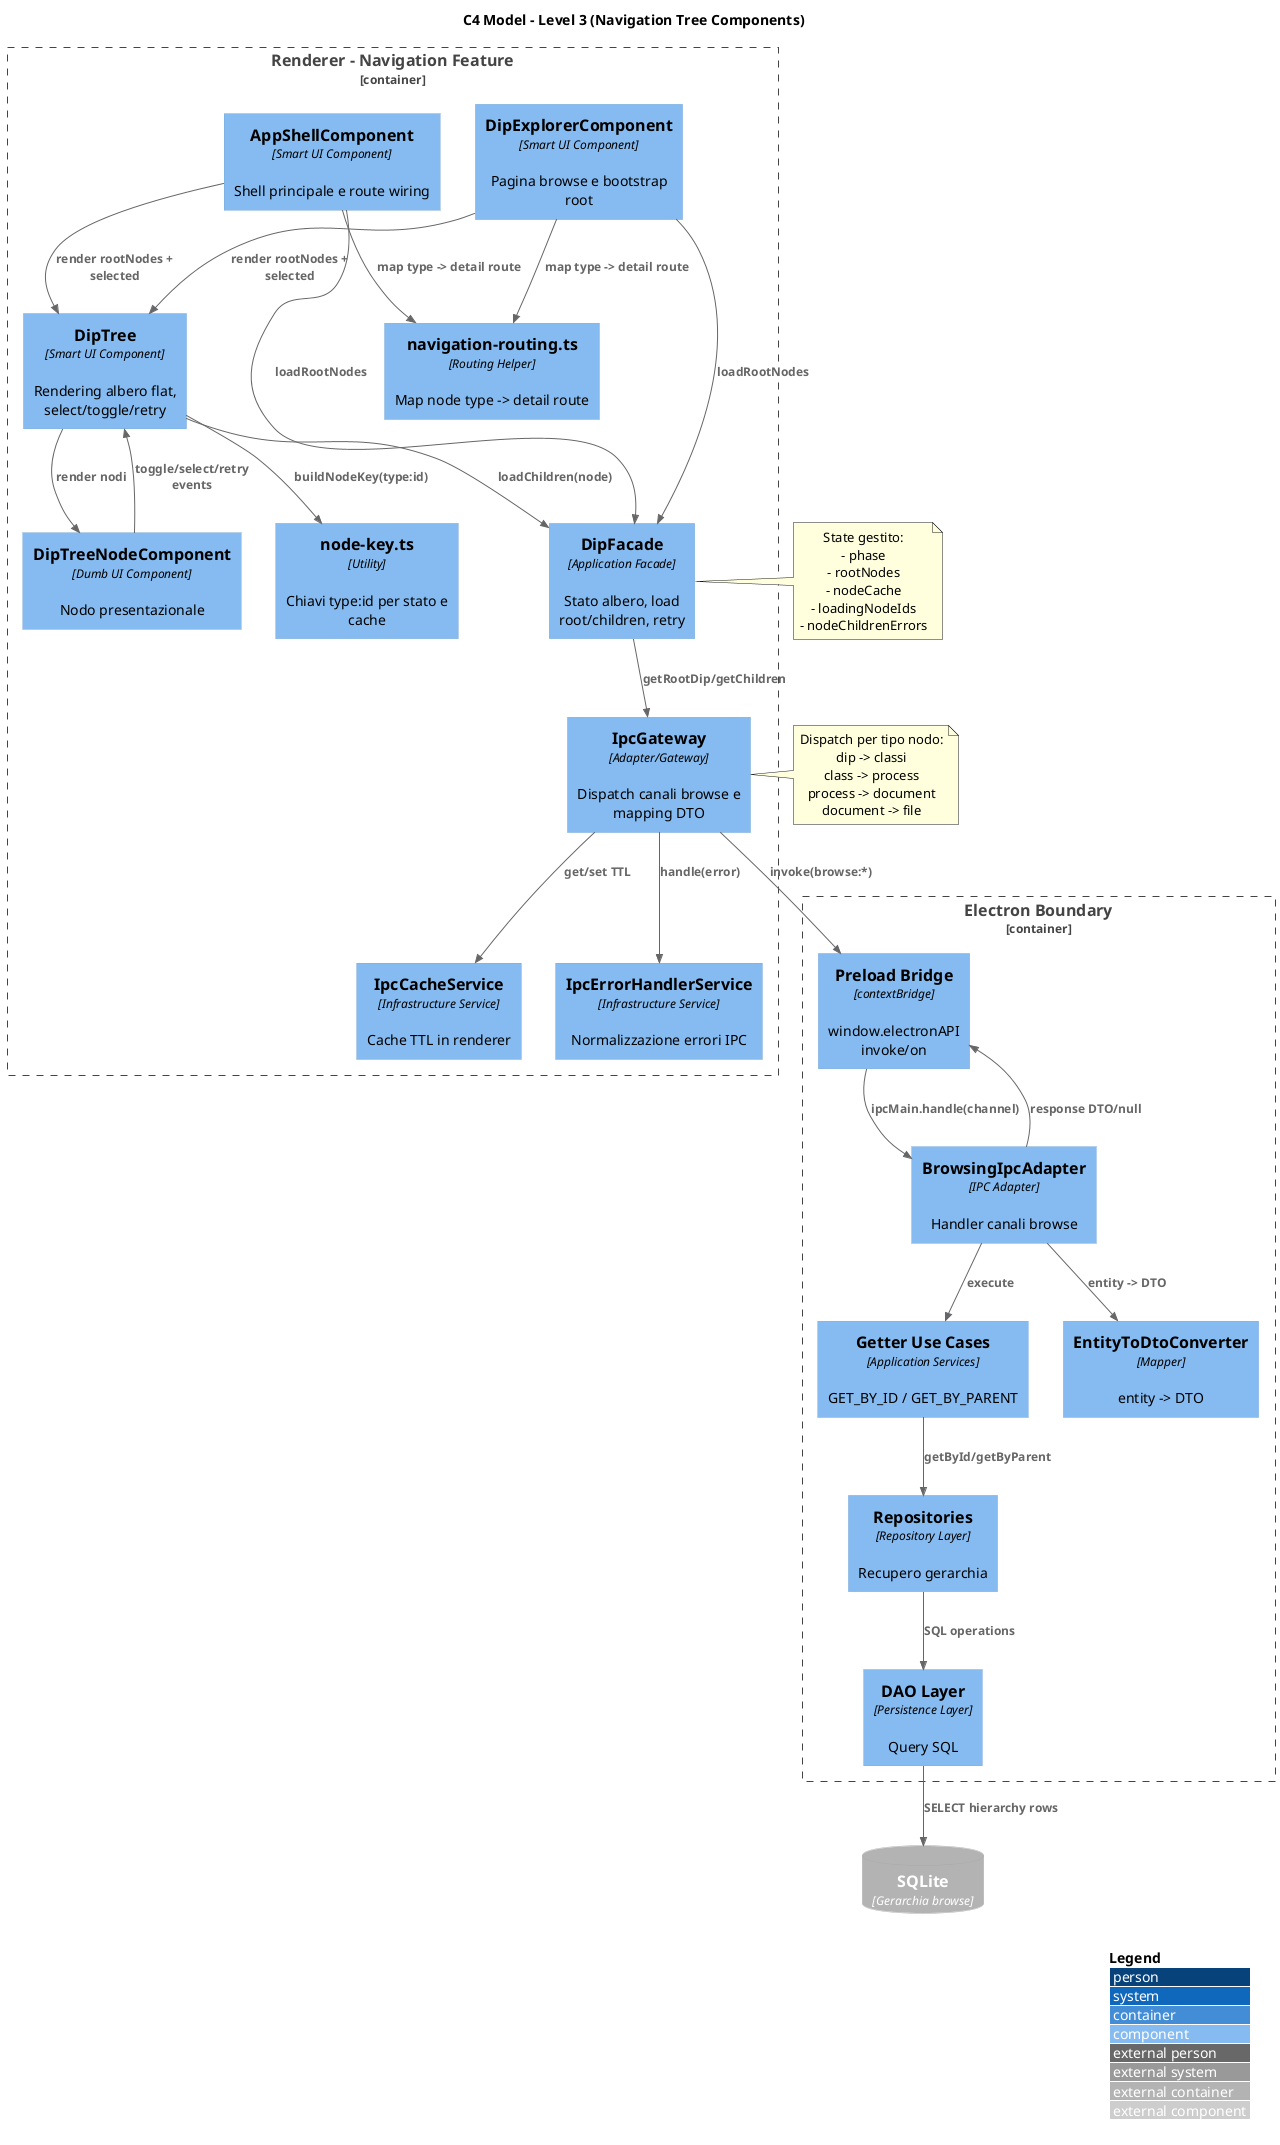
\includegraphics[width=0.9\textwidth]{../../assets/outDiagrammiST/C4_Navigation_Component.png}
	\caption{Diagramma C3 - Component View del modulo Albero di Navigazione}
	\label{fig:navigation:c3-component}
\end{figure}

\subsubsection{Architettura del modulo}

\begin{table}[H]
	\centering
	\footnotesize
	\setlength{\tabcolsep}{4pt}
	\renewcommand{\arraystretch}{1.35}
	\begin{tabularx}{\textwidth}{|l|l|Y|}
		\hline
		\textbf{Layer} & \textbf{Componente} & \textbf{Responsabilita} \\
		\hline
		Renderer & \texttt{DipFacade} & Stato albero (phase, rootNodes, nodeCache, loadingNodeIds, nodeChildrenErrors), orchestrazione load root/children, retry e gestione errori. \\
		\hline
		Renderer & \texttt{IpcGateway} & Dispatch canali browse per tipo nodo, mapping DTO -> DipTreeNode, cache TTL, fallback naming. \\
		\hline
		Renderer & \texttt{DipTree} / \texttt{DipTreeNodeComponent} & Rendering albero flat, espansione/collasso, selezione nodo e retry locale. \\
		\hline
		Renderer & \texttt{AppShellComponent} / \texttt{DipExplorerComponent} & Bootstrap root nodes e integrazione con il routing di dettaglio. \\
		\hline
		Renderer & \texttt{navigation-routing.ts} / \texttt{node-key.ts} & Mapping tipo nodo -> route dettaglio e chiave composta \texttt{type:id} per cache/stato. \\
		\hline
		Backend & \texttt{preload.ts} / \texttt{main.ts} & Boundary Electron, allowlist canali, bridge invoke/on e registrazione adapter IPC. \\
		\hline
		Backend & \texttt{BrowsingIpcAdapter} + UseCase + Repository + DAO & Esecuzione query browse su SQLite e conversione entity -> DTO. \\
		\hline
	\end{tabularx}
	\caption{Architettura tecnica del modulo Navigazione}
	\label{tab:navigation:arch}
\end{table}

\subsubsection{Flussi operativi principali}

\paragraph{Bootstrap albero root}
\begin{enumerate}[labelwidth=0.8cm,leftmargin=1cm]
	\item \texttt{AppShellComponent} o \texttt{DipExplorerComponent} avvia l'inizializzazione dei nodi root.
	\item \texttt{DipFacade.loadRootNodes(dipId)} imposta \texttt{phase=loading}.
	\item \texttt{IpcGateway.getRootDip} invoca \texttt{BROWSE\_GET\_DIP\_BY\_ID}.
	\item Il backend risolve la richiesta via \texttt{BrowsingIpcAdapter} e catena UseCase -> Repository -> DAO.
	\item La facade aggiorna \texttt{phase=ready} e popola \texttt{rootNodes}.
\end{enumerate}

\paragraph{Espansione nodo}
\begin{enumerate}[labelwidth=0.8cm,leftmargin=1cm]
	\item \texttt{DipTree.toggleNode(node)} marca il nodo come espanso/collassato.
	\item Se il nodo non e in cache, \texttt{DipFacade.loadChildren(node)} avvia il caricamento.
	\item La facade aggiorna \texttt{loadingNodeIds} e pulisce eventuali errori pregressi sul nodo.
	\item \texttt{IpcGateway.getChildren} effettua dispatch per tipo nodo:
	\begin{itemize}
		\item dip -> \texttt{BROWSE\_GET\_DOCUMENT\_CLASS\_BY\_DIP\_ID}
		\item documentClass -> \texttt{BROWSE\_GET\_PROCESS\_BY\_DOCUMENT\_CLASS}
		\item process -> \texttt{BROWSE\_GET\_DOCUMENTS\_BY\_PROCESS}
		\item document -> \texttt{BROWSE\_GET\_FILE\_BY\_DOCUMENT}
		\item file -> nessun figlio
	\end{itemize}
	\item Al successo i figli sono salvati in \texttt{nodeCache}; al fallimento in \texttt{nodeChildrenErrors}.
\end{enumerate}

\paragraph{Selezione nodo e routing}
\begin{enumerate}[labelwidth=0.8cm,leftmargin=1cm]
	\item \texttt{DipTree.selectNode(node)} emette \texttt{nodeSelected}.
	\item AppShell/DipExplorer mappano il tipo nodo con \texttt{mapDipNodeTypeToDetailItemType()}.
	\item \texttt{buildDetailRoute(itemType, node.id)} costruisce la route target.
	\item Angular Router naviga verso \texttt{/detail/:itemType/:itemId}.
\end{enumerate}

\subsubsection{Contratti principali}

\paragraph{Stato della DipFacade}
\begin{itemize}
	\item \texttt{phase}: stato globale della feature (\texttt{ready|loading|idle}).
	\item \texttt{rootNodes}: nodi radice mostrati in albero.
	\item \texttt{nodeCache}: figli gia caricati per parent.
	\item \texttt{loadingNodeIds}: set dei nodi in caricamento.
	\item \texttt{nodeChildrenErrors}: errori locali per nodo.
	\item \texttt{rootError}: errore di bootstrap root.
\end{itemize}

\paragraph{Nodo di navigazione}
\begin{itemize}
	\item \texttt{name: string}
	\item \texttt{id: number}
	\item \texttt{type: dip|documentClass|process|document|file}
	\item \texttt{hasChildren: boolean}
	\item \texttt{timestamp?: string}
\end{itemize}

\paragraph{Firme metodi chiave}
\begin{itemize}
	\item \texttt{DipFacade.getState()}\\
	\texttt{: Signal<DipState>}
	\item \texttt{DipFacade.loadRootNodes(dipId: number)}\\
	\texttt{: Promise<void>}
	\item \texttt{DipFacade.loadChildren(target: number}\\
	\texttt{| DipTreeNode): Promise<void>}
	\item \texttt{IpcGateway.getRootDip(dipId: number)}\\
	\texttt{: Promise<DipTreeNode>}
	\item \texttt{IpcGateway.getChildren(parent: DipTreeNode)}\\
	\texttt{: Promise<DipTreeNode[]>}
	\item \texttt{DipTree.toggleNode(node: DipTreeNode)}\\
	\texttt{: void}
	\item \texttt{DipTree.retryNode(node: DipTreeNode)}\\
	\texttt{: void}
	\item \texttt{DipTree.selectNode(node: DipTreeNode)}\\
	\texttt{: void}
\end{itemize}

\subsubsection{Canali IPC usati}

\begin{table}[H]
	\centering
	\footnotesize
	\setlength{\tabcolsep}{4pt}
	\renewcommand{\arraystretch}{1.35}
	\begin{adjustbox}{max width=\textwidth}
	\begin{tabular}{|l|l|l|l|}
		\hline
		\textbf{Costante} & \textbf{Canale} & \textbf{Payload} & \textbf{Return} \\
		\hline
		\texttt{BROWSE\_GET\_DIP\_BY\_ID} & \texttt{browse:get-dip-by-id} & \texttt{id:number} & \texttt{DipDTO | null} \\
		\hline
		\texttt{BROWSE\_GET\_DOCUMENT\_CLASS\_BY\_DIP\_ID} & \texttt{browse:get-document-class-by-dip-id} & \texttt{dipId:number} & \texttt{DocumentClassDTO[]} \\
		\hline
		\texttt{BROWSE\_GET\_PROCESS\_BY\_DOCUMENT\_CLASS} & \texttt{browse:get-process-by-document-class} & \texttt{documentClassId:number} & \texttt{ProcessDTO[]} \\
		\hline
		\texttt{BROWSE\_GET\_DOCUMENTS\_BY\_PROCESS} & \texttt{browse:get-documents-by-process} & \texttt{processId:number} & \texttt{DocumentDTO[]} \\
		\hline
		\texttt{BROWSE\_GET\_FILE\_BY\_DOCUMENT} & \texttt{browse:get-file-by-document} & \texttt{documentId:number} & \texttt{FileDTO[]} \\
		\hline
	\end{tabular}
	\end{adjustbox}
	\caption{Canali IPC utilizzati dal modulo Navigazione}
	\label{tab:navigation:ipc}
\end{table}

\subsubsection{Cache, naming e gestione errori}

\paragraph{Cache}
\begin{itemize}
	\item Cache nel renderer tramite \texttt{IpcCacheService}.
	\item TTL del gateway: \texttt{600000 ms}.
	\item Chiave nodo composta: \texttt{type:id}.
	\item Strutture correlate: \texttt{nodeCache}, \texttt{loadingNodeIds}, \texttt{nodeChildrenErrors}.
\end{itemize}

\paragraph{Naming}
\begin{itemize}
	\item Uso del nome preferito da DTO/metadata quando disponibile.
	\item Fallback per tipo nodo (DIP, Classe Documentale, Processo, Documento, File).
	\item Normalizzazione filename per i nodi file (ultimo segmento path).
\end{itemize}

\paragraph{Error handling}
\begin{itemize}
	\item Errori root: \texttt{rootError} e \texttt{phase=idle}.
	\item Errori figli: isolamento per nodo in \texttt{nodeChildrenErrors}.
	\item Retry nodo dedicato senza bloccare altri rami dell'albero.
	\item Normalizzazione errori IPC tramite \texttt{IpcErrorHandlerService}.
\end{itemize}
